% !TEX TS-program = XeLaTeX

\documentclass[12pt, notitlepage,
%draft
]{ctexbook}
\usepackage{xeCJK}
\usepackage[font=small]{caption, subcaption}
\usepackage{tikz}
\usepackage{fancyhdr}
\usepackage{amsmath}
\usepackage{graphicx}
\usepackage{xcoffins}
\usepackage{xcolor}
\usepackage{fontspec}
\usepackage[a4paper]{geometry}
\usepackage{setspace}
\usepackage{emptypage}
\usepackage{titlesec}
\usepackage[breaklinks,colorlinks,linkcolor=black,citecolor=black,urlcolor=black]{hyperref}
% Set up commands for title page generation
\definecolor{ethblue}{RGB}{31, 64, 122}


\newfontfamily\dinprobold{HBLiXuKeShuFa}
\newCJKfontfamily\cnprobold{HBLiXuKeShuFa}
\newCJKfontfamily\cnproregular{HBLiXuKeShuFa}
\newCJKfontfamily\cnprolight{KaiTi}
\graphicspath{ {images/} }
\newcommand\mypar{\vspace{1em} \par}
\newcommand\chapterdecoration{%
	\begin{tikzpicture}[remember picture,overlay,shorten >= -10pt]
	\filldraw[black,line width=0,rounded corners=0] (0,2.5) rectangle (\linewidth,2.55);
	\end{tikzpicture}%
}
\titleformat{\chapter}[display]%
{\heiti\zihao{1}}%
{第\zhnumber\thechapter 章}{10pt}%
{}[\vspace*{2cm}\chapterdecoration]

\begin{document}

	\pagestyle{empty}
	\NewCoffin \result
\NewCoffin \anchor
\NewCoffin \topbox
\NewCoffin \ethlogo
\NewCoffin \imagebox
\NewCoffin \textbox
\NewCoffin \departmentlogo
\NewCoffin \textboxtext
\NewCoffin \textboxsubtext
\NewCoffin \authortext

\SetHorizontalCoffin \result {}
\SetHorizontalCoffin \topbox {\color{ethblue}\rule{220mm}{3cm}}
\SetHorizontalCoffin \imagebox {\includegraphics[width=190mm]{haupt}}
%\SetHorizontalCoffin \ethlogo {\includegraphics[width=50mm]{ethlogo}}
\SetHorizontalCoffin \textbox {\color{ethblue}\rule{190mm}{100mm}}
\SetVerticalCoffin \textboxtext {160mm} {\fontsize{60}{72}\cnprobold\noindent\textcolor{white}{\dinprobold{CDAI} 文化指南}}
\SetVerticalCoffin \textboxsubtext {160mm} {\fontsize{21}{25}\cnproregular\noindent\textcolor{white}{——中德文化差异小百科}}
\SetVerticalCoffin \authortext {160mm} {\flushright\fontsize{10}{12}\cnprolight\noindent\textcolor{white}{中德工程师学院}}
\SetHorizontalCoffin \departmentlogo {\includegraphics[width=30mm]{logo}}

% Positioning Hax
\JoinCoffins \result \topbox
\JoinCoffins \result[\topbox-hc, \topbox-b] \imagebox [hc, t](0mm,10mm)
\JoinCoffins \result[\imagebox-l, \imagebox-t] \ethlogo [l, b](0mm,5mm)
\JoinCoffins \result[\imagebox-l, \imagebox-b] \textbox [l, t](0mm,0mm)
\JoinCoffins \result[\textbox-hc, \textbox-t] \textboxtext [hc, t](-5mm, -5mm)
\JoinCoffins \result[\textboxtext-l, \textboxtext-b] \textboxsubtext [l, t](0mm, -5mm)
\JoinCoffins \result[\textbox-r, \textbox-b] \authortext [r, b](-5mm, 5mm)
\JoinCoffins \result[\textbox-l, \textbox-b] \departmentlogo [l, t](-5mm, -5mm)


% Generate the page
\thispagestyle{empty}
\newgeometry{left=0mm,bottom=0mm, top=0mm, right=0mm}
\noindent\TypesetCoffin \result
\restoregeometry
	\cleardoublepage
	\thispagestyle{empty}
	\begin{titlepage}
	\newgeometry{bindingoffset=0cm,left=3cm,right=3cm}
	
	%\vspace*{8cm}
	\noindent
	\center
	\begin{minipage}{\linewidth}
	%\zihao{0}\heiti CDAI文化指南\par
	\fontsize{60}{72}\cnprobold{\dinprobold{CDAI}文化指南}\par
	\vspace{12pt}
	%\zihao{-2}\songti ——中德文化差异百科\par
	\fontsize{21}{25}\cnproregular{——中德文化差异小百科}\par
	\vspace{8cm}
	\heiti\zihao{-3}
	%\includegraphics{logo}
	\raggedright
	项目成员:\\
	
	\vspace*{1em}
	\zihao{4}
	黄伟根\\
	黄耀鑫 \hspace{1em} 杨星林 \hspace{1em} 詹均升 \\
	张嘉伟 \hspace{1em} 周功豪 \hspace{1em} 周鹏 \\
	\end{minipage}
	\vfill
	\zihao{3}\cnprolight{中德工程师学院}\par
	\href{http://cdai.zust.edu.cn/}{\texttt{http://cdai.zust.edu.cn/}}
	\end{titlepage}

	\cleardoublepage
	\vspace*{3cm}
\begin{minipage}{\linewidth}
    \Huge\heiti\center{封面图片} \par
\end{minipage}

 \vspace*{3cm}

\par
勃兰登堡门位于德国首都柏林的市中心,最初是柏林城墙的一道城门,因通往勃莱登堡而得名。现在保存的勃莱登堡门是一座古典复兴建筑,由普鲁士国王腓特烈·威廉二世下令于1788年至1791年间建造,以纪念普鲁士在七年战争取得的胜利。
\cleardoublepage

\begin{minipage}{\linewidth}
\Huge\heiti\center{关于本书} \par
\end{minipage}

\vspace*{3cm}
 %\normalfont\normalsize
 %\raggedright
 %\indent
中国和德国都是世界上具有重大影响力的国家,随着传播 通讯技术的改进,交通技术的进步和经济的高度全球化,两国的合作越来越频繁。 然而,由于文化背景的不同,中德两国人民在文化交流上还略有欠缺。针对中德工程师学院和德国的应用技术大学之间日益频繁的交流活动,作为中德工程师学院的学生我们希望将一些所闻所知的信息整理、归类,尽可能为两国的学生了解对方文化提供一些一些帮助。本书不求包罗万象,但求准确,详尽,有趣。

\par
在上学期,我们小组成员在项目发起人Frau Schneider的引领和指导下,为了增进我院及合作院校中、德两国学生间的文化认同感,减轻乃至消除文化差异所带来的沟通障碍,同时也为了我院新生能够更快适应和融入国际化的教学方式,多元化的人文环境,开展了一系列关于中德文化差异的研讨会、采访、问卷调查和现场调研。我们最终决定将项目的视角聚焦在七个文化主题上:服饰、饮食、体育、工作、交通、文化、卫生,以Wiki为载体,配以百科全书式的写作手法,从学生的视角出发,独特地展现出我们对于异国文化的认识与思考。在项目期间,我们充分运用所学项目管理的知识,通过Projekt Auftrag, Zeitplan, PSP等项目管理工具精确的控制项目进程;通过查阅相关资料、与德国师生互相交流讨论,并结合实际的生活体验,确定了各项主题的具体内容,并定期向同学与老师展示工作成果。项目的最后,我们的成果是喜人的,我们的中德文化差异百科全书在学院官网上线,向中德师生展现了中德文化大花园的一隅,虽然项目仍有不少改进的空间,但是我们希望通过这个学期的共同努力,把中德文化差异百科这座文化桥梁打造的更加坚固、优美。 相比于上学期, 这学期我们将从中德两国人民的日常行为差异入手,深入分析每个差异代表的文化内涵。我们希望通过这些方法,使中德两国国学生增进理解,弥合文化差异的鸿沟。
\par
在中国有一个小故事,讲的是汉朝的时候,在西南方有个名叫夜郎的小国家,它虽然是一个独立的国家,可是国土很小,百姓也少,物产更是少得可怜。但是由于邻近地区以夜郎这个国家最大,从没离开过国家的夜郎国国王就以为自己统治的国家是全天下最大的国家。有一天,夜郎国国王与部下巡视国境的时候,他指着前方问说:“这里哪个国家最大呀?”部下们为了迎合国王的心意,于是就说:“当然是夜郎国最大啰!”走着走着,国王又抬起头来、望着前方的高山问说:“天底下还有比这座山更高的山吗?”部下们回答说:“天底下没有比这座山更高的山了。”后来,他们来到河边,国王又问:“我认为这可是世界上最长的河川了。”部下们仍然异口同声回答说:“大王说得一点都没错。”从此以后,无知的国王就更相信夜郎是天底下最大的国家。有一次,汉朝派使者来到夜郎,途中先经过夜郎的邻国滇国,滇王问使者:“汉朝和我的国家比起来哪个大?”使者一听吓了一跳,他没想到这个小国家,竟然无知的自以为能与汉朝相比。却没想到后来使者到了夜郎国,骄傲又无知的国王因为不知道自己统治的国家只和汉朝的一个县差不多大,竟然不知天高地厚也问使者:“汉朝和我的国家哪个大?”。夜郎国王固然可笑,但如果我们固步自封坐井观天岂不是跟夜郎国王一样。
\par
在如今全球化的背景下,中国青年更应该睁眼看世界,走出国门拥抱世界。德国作为世界上数一数二的大国。德国文化更是不可忽视的。面对中德两国日益平凡的交流,德国青年对中国文化越来越有兴趣。总之,这本小册子希望可以作为两国学生了解对方文化的起点。作为中国学生我们对德国文化没有更深入的了解,在此也欢迎正在看此书的你,提出宝贵的建议。
\par
\vspace{\baselineskip} 
\hfill {\heiti 2019年三月,杭州}

	\tableofcontents

	\pagestyle{headings}	
	\input{Essen/Essen}
	\chapter{节日文化差异}
在德国提到节日可以说“Fest”、“Festival”以及“Feiertag”,对应中国的来说可以是节日和法定假日,“Festival”一般是在某个城市或小镇举办的音乐节或是狂欢节。对于中国人来说法定假日的数量不多,更多的是拼假组成的黄金周。
\input{Festival/Traditionelles_Festival}
\section{政治性节日}

\subsection{马丁·路德宗教改革日}

每年10月31日,五个德国州聚集在一起庆祝宗教改革日。随着这个国家动荡而微妙的历史,人们可能会想知道庆祝的是哪个改革活动,或者为什么只有大约三分之一的国家在庆祝。旨在回答这些问题以及更多问题,这里有一段德国宗教改革日的简史。宗教改革日是观察新教改革的官方公共假日,由德国僧侣马丁·路德颁布。具体来说,德国的宗教改革日标志着他在1517年将他著名的95篇论文钉在维滕贝格教堂门口的周年纪念日。他在11月1日万圣节前夕这样做,因为他知道许多人会聚集在教堂,这确保了他的论文的最大可见性。路德最感兴趣的是废除出售赎罪券作为寻求赎罪的手段。在路德的时代,众所周知,这笔钱被用来资助罗马圣彼得大教堂的翻修,这说明了出售放纵品的做法有多腐败。然而,95篇论文列出了路德对教会怀有的许多其他不满。这一重大事件给德国和其他国家带来了重大变化,因为路德教和其他新教派别开始反对天主教会,在这些抗议活动发生时,天主教会确实变得相当专制。当路德用拉丁文写这些论文时,这些论文被迅速翻译成德语,并在全国和其他地方广泛传播。改革时期在随后的一个世纪里以重要的社会、历史和宗教方式进行,直到1648年。宗教改革浪潮中出现了多个新教教派,教会在人民生活中调解上帝存在的作用受到了彻底的审视。早在1567年,各个教派的新教教会每年秋季都举行一天的活动,纪念95篇论文的发表。然而,在当代,在大多数地方,宗教改革日是在10月31日。每年,德国的州一级都会庆祝这个节日。包括勃兰登堡州、萨克森州、梅克伦堡西波美拉尼亚州、图林根州和萨克森安哈尔特州在内的五个州是该国宗教改革日为官方假日的地方。这五个州在历史上都是新教徒,在95篇论文发表后,社会和文化生活发生了重大变化。今天,这些地区通过给人们放假来纪念宗教改革日。此外,为纪念这一天,银行和邮局等公共机构也关闭了。在这些地方和其他地方,路德教会和改革派教会经常举行特别纪念活动。用来代表这一天的象征性颜色是红色,这是针对圣灵的。赞美诗《强大的堡垒是我们的上帝》通常是为了向写这首诗的路德致敬而唱的。为了纪念路德,许多面包、蛋糕和甜食也在这一天传统上被消费。

马丁·路德宗教改革出现的根本原因是随着西欧商品经济和资本主义的发展,天主教会成为资本主义发展的最大障碍,专制君主、银行家和商人、中小贵族、新兴资产阶级、下层贫民,都想通过反对教会来改善自己的经济状况。对德国的影响有推动了广大民众的反封建斗争,沉重打击了天主教会和封建势力,有利于德意志民族语言的发展,并为欧洲的其他国家和地区的宗教改革开辟了道路。那么在宗教改革日那天德国人会做些什么呢?每年10月31日,五个德国州聚集在一起庆祝宗教改革日。随着这个国家动荡而微妙的历史,人们可能会想知道庆祝的是哪个改革活动,或者为什么只有大约三分之一的国家在庆祝。旨在回答这些问题以及更多问题,这里有一段德国宗教改革日的简史。宗教改革日是观察新教改革的官方公共假日,由德国僧侣马丁·路德颁布。具体来说,德国的宗教改革日标志着他在1517年将他著名的95篇论文钉在维滕贝格教堂门口的周年纪念日。包括勃兰登堡州、萨克森州、梅克伦堡西波美拉尼亚州、图林根州和萨克森安哈尔特州在内的五个州是该国宗教改革日为官方假日的地方。今天,这些地区通过给人们放假来纪念宗教改革日。此外,为纪念这一天,银行和邮局等公共机构也关闭了。在这些地方和其他地方,路德教会和改革派教会经常举行特别纪念活动。用来代表这一天的象征性颜色是红色,这是针对圣灵的。赞美诗《强大的堡垒是我们的上帝》通常是为了向写这首诗的路德致敬而唱的。为了纪念路德,许多面包、蛋糕和甜食也在这一天传统上被消费。

\paragraph{马丁·路德的故事}
路德在1517年万灵节前夕,也就是十月三十一日那天,宣布他反对赎罪券,写了九十五条论纲。其实这九十五条的目的并非是号召宗教改革,只是路德以一位大学教授的身份将赎罪券的神学提出来讨论罢了。路德反对赎罪券的曲解和误用,这不但对人的得救不利,还影响了教会的正常运作。当时的人们认为天国的钥匙在教会手里,一个人进入天堂前要先洗清生前所犯的一切罪行。他们最怕的是死后在炼狱中的刑罚,因此他们相信只要用赎罪券就可以上天堂,一张赎罪卷能缩短死后在炼狱中的刑罚。而赎罪劵可以在教堂里购买,因此当时的教堂和牧师都很有钱。马丁路德发现这样的说法与作法完全不能见容于圣经与理性。赎罪券的买卖鼓励了处于罪恶中的人,不去思想基督,不去祈求上帝的饶恕。就这一点,路德的神学与天主教会的神学有明显的不同。1530年路德在奥斯堡会议上为新运动作了解释,他的改教运动已把基督教欧洲一分为二,更正教会产生了三个主要路线:信义宗、改革宗和英国圣公宗。更正教会主张信徒应该直接和基督联合,因为基督是救恩的唯一来源。他的救恩借着圣灵的能力和上帝的道的教导,临到悔改的信徒。路德的宗教改革受到四面攻击。罗马教廷要路德收回他的言论和著作,路德并没有答应。在他隐居于瓦尔特堡(Wartburg)那段日子里,路德把整本新约圣经由希腊文译成精彩的德文。在那期间,左派极端的社会行动到处兴事,路德于是回到威登堡以稳定大学和教会的生活,并且应付四面八方涌来的攻击。甚至有的人民误解了路德说的自由,牵扯到政治,拿了武器去争取,造成了改教运动的致命伤。路德被罗马教会定罪,逐出教会。
\begin{figure}[htb]
    \centering
    
\includegraphics[width=0.6\linewidth]{mdld}
    \caption{马丁路德}
    
\end{figure}

\subsection{妇女节}

创立国际劳动妇女节的主要提议者:克拉拉·蔡特金(Clara Zetkin,1857.7.5-1933.6.20),原名克拉拉·艾斯纳,德国社会民主党和第二国际左派领袖之一,国际社会主义妇女运动领袖之一,德国共产党创始人之一,无产阶级女权解放的灵魂人物。1910年8月,蔡特金在丹麦首都哥本哈根召开了国际社会主义者第二次妇女代表大会。倡议以每年的3月8日作为全世界妇女的斗争日,1911年的3月8日为第一个国际劳动妇女节。“三八”妇女节成为世界妇女争取权利、争取解放的节日。

在德国柏林地区,妇女节是法定假期,全天休假。

\subsubsection{妇女节在中国 ——三八红旗手}
是中国在三月八号妇女节颁给优秀劳动妇女的荣誉称号,主要是表彰在中国各条战线上为社会主义物质文明和精神文明建设做出显著成绩的妇女先进人物和妇女先进集体

\paragraph{政治背景}
中华人民共和国成立后,鼓励妇女进入工厂工作,离开传统的家庭区。 它们主要被视为工作的来源,因此是一个在文化领域,特别是当时的政治宣传方面出现充满力量感的女性形象。
\begin{figure}[htb]
    \centering
    \includegraphics[width=0.3\linewidth]{frau1}
    \includegraphics[width=0.3\linewidth]{frau2}
    
    \includegraphics[width=0.3\linewidth]{frau3}
    \includegraphics[width=0.3\linewidth]{frau4}
    \caption{中国曾经的政治宣传画}
\end{figure}
\input{Festival/Regionales_Festival}
\section{节日禁忌} 
\begin{figure}[htb]
    \centering
    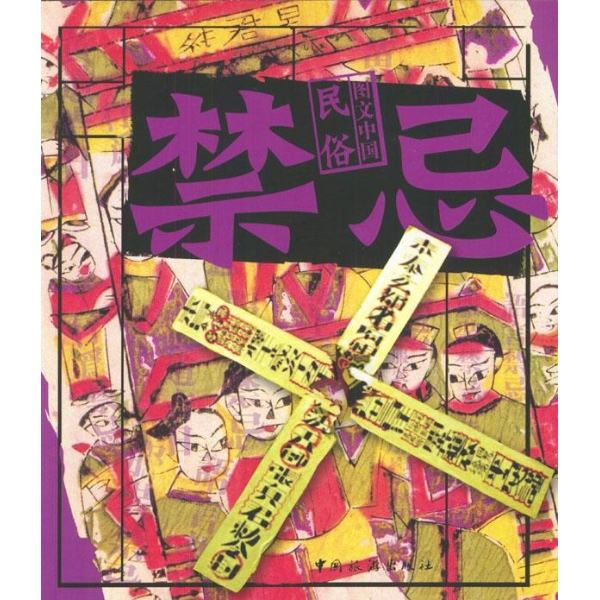
\includegraphics[width=0.5\linewidth]{jinji}
    \caption{节日禁忌}
    
\end{figure}

    “禁忌”一词来源于,国际学术界统称为“塔布”,源于太平洋小岛波利尼西亚汤加岛人的土语,音译为“taboo”或“Tabu”,其基本含义是表示“神圣的”、“不洁的”、和“危险的”、“不可接触的”。
    中国文化博大精深,然而在中国的传统文化当中有很多的禁忌,如果按照老一辈的人来说,这是老天爷安排的。按照现代人说,这就是迷信。但是无论是迷信是否,作文中国文化,我们更应该用继承的心态去面对。下面就介绍一些中国人在日常生活中碰到的或是不愿意去犯的禁忌。



\subsection{送礼禁忌}

    相信不止大家都为了挑选礼物而烦恼过,面对各种各样的节日,我们总是需要不停的购买适当的礼物送给对应的人,这个真的很让人苦恼。但是亲朋好友之间互相送礼物,更多的是为了传达一种祝福、表达一种诚意。用最近火热的词来说,就是一种“仪式感”。你挑选的礼物不一定真的符合你送礼对象的心意,或者也不是他们真正需要的。给同样的钱让他们自己买他们或许也不会买这个礼物,甚至你礼物送出去之后他们一辈子都不一定会用上一次。然而你在挑选礼物的过程中,已经投入了大量的精力和时间,而正是这些东西,会让对方感受到你的心意,这就是所谓的“礼轻情意重。”所以但是根据中国的风俗传统,送以下系类的礼物却可能会导致好心做坏事,也是众多礼物中比较忌讳的礼物:

    \begin{enumerate}
   \item 
   送结婚礼物时忌讳送“伞”、“钟”等物,因为“伞”与“散”谐音,散意离散,为人们所不喜欢,所以伞被视为不吉利的礼物,“钟”与“终”谐音,特别是“送钟”更会让老人们联想到“送终”,很不吉利。
   \item
   给病人送食品时也有谐音的禁忌。旧时上海去看望病人时,忌送苹果,因为上海话中“苹果”的发音与“病故”谐音。
   \item
   菊花常用于纪念逝者,不可以作为礼物送出。
   \item
   帽子俗话中有“愁帽子”之说,老人去世孝子要头戴孝帽,所以忌讳将帽子送给别人。特别是绿色的帽子,更是送礼的大忌。
   \item
   刀剑等利器,容易伤人,且俗话有“一刀两断”之说,用于送人恐有割断关系双方的不好联想,所以一般不作为礼品送人。
   \item
   扇子因为只用于夏天,一到秋凉天即被抛之不用,有绝情之意,俗称“送扇无相见”,所以不受欢迎,而且很多人会将“风扇”当成“分散”理解,潜台词就是分手。
   \item
   “鞋”与“邪”同音,而且鞋被踩在脚下,所以除了自己家人,一般不要给别人送鞋。
   \begin{figure}[htb]
    \centering
    
\includegraphics[width=0.5\linewidth]{jinjifs}
    \caption{禁忌风水}
    
    \end{figure}
   \item
   ”梨“因为“梨”与“离”谐音,给夫妻、恋人不能送就很不适合。
   \item
   “镜子”与“禁子”谐音,且镜子易破易碎,所以也属于属送礼的忌讳之物。
   
  
        
    \end{enumerate}


\subsection{数字禁忌}

    数字不仅仅可以代表数量,还关联着不同语言文化、宗教信仰等深刻内涵。不同的国家地区都有着不同的数字禁忌,也有着不一样的数字偏好。如中国人就忌讳4,偏爱6、8、9。
    \begin{enumerate}
    \item 
    “四”谐音“死”,大凶,所以门牌号、车牌号都不宜有这个数字。过年的时候也忌说“4”、“死”等音的词。在日常生活中也能看到这样的例子:有很多外国人在中国生活久了之后都清楚在中国绝大部分大厦中是没有“4楼”的存在,通常是用“3A楼”或者“5A楼”来代替,或者直接就没有这一层楼,直接跳到了5楼。。这也是因为在中国的文字发音中间“4”和“死”同音,中国人普遍都忌讳死亡楼层。
    \item 
    数字当中,最吉利的要数六和八,所谓“六六大顺”、“要得发,不离八”,就说出了其中的原委。  
        
    \end{enumerate}
\begin{figure}[htb]
    \centering
    \includegraphics[width=0.6\linewidth]{4_Echt}
    \caption{中国常见的楼层分布}
\end{figure}


\subsection{谐音产生的禁忌}

    每年春节,全世界有超过十亿人加入庆祝的行列,并展开一场微妙的文字游戏。它很像一组求爱仪式——为了招来好运,人们会用喜庆字样的剪纸来装点住宅与门户。要理“发”的,年前赶紧理完,谁想在新年伊始削去财运,哪怕只是稍事修剪?年夜饭的菜肴里通常有鱼,因为人们希望“年年有余”;有的地方还时兴吃一种名为发菜的藻类,因为谐音“发财”;或有“橙”,寓意为“成”,所以在春节的装饰物中常常可以看见柑橘类水果的身影。而且有研究表明,在中文语境下,人们对同音歧义似乎更为敏感。
    \begin{enumerate}
    \item 
   如在亲友结婚之日,忌讳说“死、光、输、完、离、散、休”等不吉利字词。
   \item 
   在结婚时,新娘上门禁吃瓜类,因为“瓜”与“寡”谐音,以免将来做寡妇。
   \item 
   和亲友一起吃梨时不能分吃一个梨,因为“分梨”与“分离”谐音。
   \begin{figure}[htb]
    \centering
    
\includegraphics[width=0.5\linewidth]{bagua}
    \caption{阴阳八卦:在中国阴阳八卦是所有禁忌产生的根源}
    
    \end{figure}

     
    

   \item 
   沿海渔民或船家忌说“沉”、“箸”等字。因为“沉”和“沉船”的沉同音同字,因此人们把“沉”字改说“重”字。吃饭用的“箸”与“住”谐音,即停住抛锚之意,对行船来说是不吉利的。因此人们把吃饭时用的“箸”改称“筷子”,取“筷”与“快”的谐音,即“快”行、“一帆风顺”之意。
   \item 
   在广州一带,人们把“猪舌”称作“猪月利”,由于广东话中“舌”与“蚀”同音,经商者忌讳蚀本,改称“猪月利”则含“月月盈利”的意思。北京话“舌”与“折”同音,也有“折本”不吉利之嫌,因此北京、天津等地把“猪舌”称作“口条”。广州人把丝瓜称作“胜瓜”,因为广州话“丝”与“输”谐音。广东潮汕一带把“药”称作“利市”或“甘茶”,而忌说“药”字,因为“药”与“病”相关,所以把有病“服药”叫“辗利市”或“服甘茶”。
        
    \end{enumerate}

\subsection{其他}

    除了上文中的禁忌之外,中国人在日常生活中还有许多有趣的禁忌。
    \begin{enumerate}
    \item
    \textbf{在中国写别人名字的时候十分忌讳用红笔书写}

   这一点在老一辈人中间特别在意,在他们看来红色墨水写出来的字颜色接近血色,是带有诅咒的意思,如果用红色墨水写一个人的名字将会给这个人带了厄运,所以很多的老师在小学的时候就会告诉小孩子不要用红笔写名字。

   \item
   \textbf{吃饭的时候所有人都忌讳将筷子竖拆在饭碗中间}

   第二个几乎是所有中国小孩都喜欢做的事情,但是无一例外都被家长斥责过。在中国是习惯吃米饭的,不像西方国家吃饭是都是使用刀叉,在中国使用的餐具基本上都是筷子,在吃饭的时候所有人都忌讳将筷子竖拆在饭碗中间,这种现象在别人看来几乎是和祭拜死人没什么差别,所有人都十分忌讳,除此之外也不能在吃饭的时候用筷子指着别人。

   \item
   \textbf{忌讳在家里种柳树}

   柳树,想必大家都很熟悉了,一种非常漂亮的树,一条条柳条随风飘摇。但是这种树虽然很好看,但是有没有小伙伴们注意到,这么漂亮的树一般很少出现在私人庭院或是哪个企业的庭院之中。因为从古至今,在民间人们都说,柳树是极阴之物,一般很少人会去接近柳树,即便是很好看也只是站在较远的地方观赏。正因为柳树是极阴之物,所以在夜晚甚至是白天的时候,会引得很多孤魂野鬼在柳树底下吸食阴气。如果有人在柳树底下呆久了,运气不好的话很有可能被冤鬼缠上,而且在阴气较重的地方呆久了,阴气入体,轻则大病一场,重则一命呜呼。也正是柳树是嫉阴之物,所以在古代民间很多道士或是先生那里都会准备一些柳条,因为柳条是可以直接抽鬼的,就像用鞭子抽人一样,有着驱鬼的功能。

   \item
   \textbf{不能敲饭碗}

   敲碗首先会显得没有教养。比如去别人家作客,假如敲碗,那么意思就是在催主人快点,等不及了。其次是民间有种说法,说吃饭敲碗,以后生活会不好,会出去乞讨,因为乞丐要饭才敲碗。
        
   \begin{figure}[htb]
    \centering
    
\includegraphics[width=0.5\linewidth]{qlbx}
    \caption{辟邪:中国人用它驱赶不吉利的事物}
    
    \end{figure}

    \end{enumerate}



   “十里不同风,百里不同俗”,在中国,各民族、各地区都有千姿百态的民俗。民俗是民间记忆的载体,反映了普通民众在历史长河中不断发展、变化的生产、生活情境以及蕴含在其中的精神与情感,是中国传统文化的重要组成部分。中国有五千年的历史,从迷信走到了科学,但是每个地方还是有老辈人口传下来的忌讳,如人的一生以36岁为大忌,每个人到了35就不做比较危险的工作,就是做什么事都比较小心点,一直到37就可以了,很多人连36这个数字都很忌讳,买卖东西不可以出现36,少给都可以,不然准挨骂,还有很多,譬如打牌的人不可以买红色的包包,过年吃团圆饭的时候严禁别人串门,又譬如一串很忌讳的老话,正月不见鹰打鸟,二月不见狗擦裆,三月不见蛇吸雾,四月不见人成双,就是看见了就会有灾难找上门。这些中国各地在不同期间的不同的习俗和禁忌,也是非常有趣又有意义的,这也是我们民族文化传统的一部份,值得世代流传。

	\chapter{个人和集体关系}
\par
和前面两章的内容相比这一部分的内容深入到了两国文化的核心内容,有较多的政治历史有关的内容。在我看来文化差异更多的是由历史演变以及经济发展水平形成的。我们打算以个人、集体这两个概念,切入到两国文化差异的核心,比较由于地理环境的因数所导致两国人对个人和集体关系的不同思考,从历史轨迹中比较文化差异的来龙去脉。

\section{现象}

\subsection{职业选择}

专业和职业的选择通常由两个因素影响,一个是自身因素,一个是外界因素。对于自身因素,专业方面和职业上一方面是自身的能力,一方面是个人的兴趣爱好。外界因素上一方面是父母对子女的期望,一方面是社会对人产生的影响。

首先是专业选择,在我们的高中时期,大多数的学生在学习期间并没有也不会考虑对于自己以后大学的专业选择,通常是高考成绩出来,确定了分数,确定了大致的学校,再考虑专业的事情。但是大多数的人并没有什么所谓的对什么专业感兴趣这种概念,没有特定兴趣的,多是与父母交换了一下意见,再在网上或是亲戚处咨询一下选择了就业前景好的热门专业。而有特定兴趣的要是就业前景好也就与上面一样,要是是个冷门专业,可能就会在父母或者亲戚的劝说下改变自己的想法,也有少数人会坚持自己的选择。还有一部分人可能是高考分数到达了目标学校的分数,但是没有到达自己所期望的专业的分数,而又勾选了服从调剂,因此被分到冷门专业。        职业选择与专业选择也是相似。刚到了毕业的时候,大多数的学生,无论是自己还是家人,自然是希望选择待遇好,条件舒适的工作。但是这时和选择专业不同的地方就是能力的大小。专业选择时虽说也有能力的区别,但是总归有大量的与你分数相近的学习与你选择。而选择职业不一样,公司看中你的能力与学历,有能力自然是你挑公司,没有能力,大公司看不上你,小公司又没有前途甚至也可能不要你,很可能就会选择与大学专业无关的工作,可以说是涝的涝死旱的旱死。
\subsection{中国人旅游}

随着旅游业的日渐兴起,无论过不过节,在世界各地,总能看到中国人的旅游大军,分布在世界的各个角落,网上关于中国旅游的话题也是吐槽多多。那么中国人和外国人的旅游到底有什么区别呢?

中国人旅游喜欢扎堆,特别是在节假日出游,到处都是人挤人,尤其在比较有名的旅游景点,你看到的到处都是乌央乌央的人头,毫无放松旅游的感觉。就算是在国外,比如在泰国游玩拍个照的时候,看到的都是一半人和一半景。但是外敷偶人旅游,同样是在泰国,却可能完全不一样,他们大都似电影里演的那样,很休闲的躺在沙滩椅上,晒着日光浴,而旁边还放一杯鸡尾酒。

扎起中国,许多大叔大妈,爷爷奶奶旅游时都强调低价,什么叫做低价。比如说,“999”玩遍泰国,“598港澳游,全程星级酒店”的这类的低价团,都备受追捧。但实际上就算是很正规的旅游团都会存在强迫购物的项目,更不要提这种明眼人一看便知的购物团了。不过在国外旅游,完全没有低价团这件事,往往都需要付足了各种费用,在泰国和越南这种收小费的习惯,其实就是他们养出来的。

中国人旅游爱逛商业街,国内外各地景色不同,但在中国旅游人的眼中,不到商业街就不算是来到了哪里旅游,尤其是以稍老一辈人最为明显,他们不论去哪儿旅游,往往都会在当地的商场里逛一圈,不论是衣服也好,纪念品也好,都很感兴趣。

中国人旅游在国外人看来,都是不可思议的,在国内人看来也是啼笑皆非。不过,这样的旅游方式其实也是非常有意思的。我觉得,作为年轻人,年轻的时候,在选择旅游方式时可以追求点个性。但是等步入了老年,很多人一起热闹旅游也未必不是好事。

近年来,越来越多的中国人都开始讨厌“扎堆”旅游,假日前夕,总有不少人在网上抱怨未来的人流高峰,甚至发誓绝不出门。但实际上,每逢节假日,国内各个主要景点依旧人山人海,人流量永远有增无减,和网上的舆论形成鲜明对比。为什么都抱怨人多,但中国人还是喜欢到人多的地方旅游呢?这是因为从全局考虑,人多也有人多的好处。
\begin{figure}[htb]
    \centering
    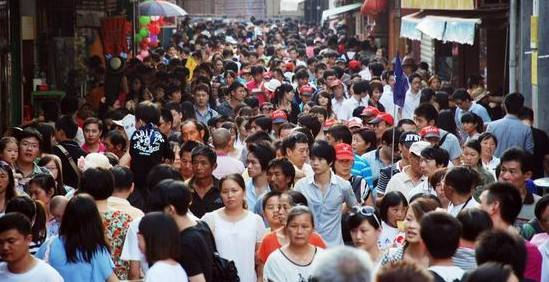
\includegraphics[width=0.6\linewidth]{zgrly}
    \caption{中国人旅游}
\end{figure}





\begin{enumerate}
    
\item \textbf{人多的地方更安全}

许多年轻的旅行者,为了规避人流高峰,喜欢挑选一些人迹罕至的地方去旅游。而人迹罕至,也就意味着这个地方充满了不可知的危险,一旦遇险,你连求援的对象都没有,只能自求多福。而人多的地方,恰恰没有这样的风险。一般来讲,热门景点都已经遭到了完全的开发,排除了大部分未知的危险因素。即便你在这些地方遭到困境,也随时可以向管理人员或身边的游客求助。过去,网上经常有驴友登山失联的消息。试想一下,如果这些山上面到处都是游客,你还会担心失联吗?事实上,在人多的地方,你想要失联都失联不了,因为没走几步,肯定会被人群挤回来。你可能会说,人多难道不是会有踩踏的危险吗?没错,但从统计数据来看,人多地方发生踩踏的概率,远远低于在荒郊野岭被野兽吃掉的概率。再比如说你的手机没电了,在人多的地方就可以很方便的借到充电宝,也是非常幸福的呀。
\begin{figure}[htb]
    \centering
    
\includegraphics[width=0.6\linewidth]{zgrly2}
    \caption{长城旅游}
\end{figure}





\item \textbf{人多的地方更温暖}

通常情况下,旅游景点的温度,都低于我们平常生活环境的温度。特别是国庆这样的节日,刚好遇到秋季,气温急剧转凉,大家从温暖的室内出来,奔赴山水之间,最大的感受就是真TMD冷。这个时候,如果你去的碰巧是荒无人烟的地方,那么很可能夜里会在帐篷里冻死。 相反,如果你去的是人流密集的场所,几万人身上散发的热量,很快就会把整个地方熏得热火朝天。

\begin{figure}[htb]
    \centering
    
\includegraphics[width=0.6\linewidth]{zgrly3}
    \caption{人多暖和}
\end{figure}



\item \textbf{人多的地方更有趣}

你去那些人群稀少的地方旅游,乍看好像无人打扰,自由自在,但很快你就会陷入空虚和无聊之中。事实上,风景永远是千遍一律的,珠峰上的景色再壮丽,让你在上面独居三十天,是个人都会崩溃。但有一种东西,永远花样翻新,永远不会腻味。没错,那就是人。正所谓“有人的地方就有江湖。”有多少个人,就有多少个江湖。而人多的经典,就好像一个浩瀚的武侠世界。在那些地方,你不仅可以看到美景,而且可以看到身边频频上演的江湖大戏,像情侣吵架、兄弟相争之类的剧目,在景点里随处可见。当然现在最流行的剧目,则是低价旅行团里导游和团客的斗争,揉和了爱情、动作、政治、商战和反乌托邦元素,倍受观众欢迎。去人多的地方旅行,“既是自然之旅,也是人文之旅。”
\begin{figure}[htb]
    \centering
    
\includegraphics[width=0.6\linewidth]{zgrly4}
    \caption{人多有趣}
\end{figure}


\item \textbf{主要是从众心理作崽}

中国人素来有凑热闹的传统,只是名气大的地方总想也去打卡一番,即使回来不停吐槽也在所不惜。这类游客通常只是喜欢出去玩,但对旅行的认知并没有到很深的层面,除了被其他人走烂的景点,别的地方都没有什么印象。
\end{enumerate}

\subsection{德国人不同于中国人的旅游方式}

生活不止眼前的苟且,还有诗和远方--- 德国人深谙这个道理,在忙碌的工作后安排一场放松身心的旅行对他们来说必不可少。2015年,德国人的度假天数总计高达8.7亿天,由此可知这是一个个酷爱度假的民族。

\begin{figure}
    \centering
    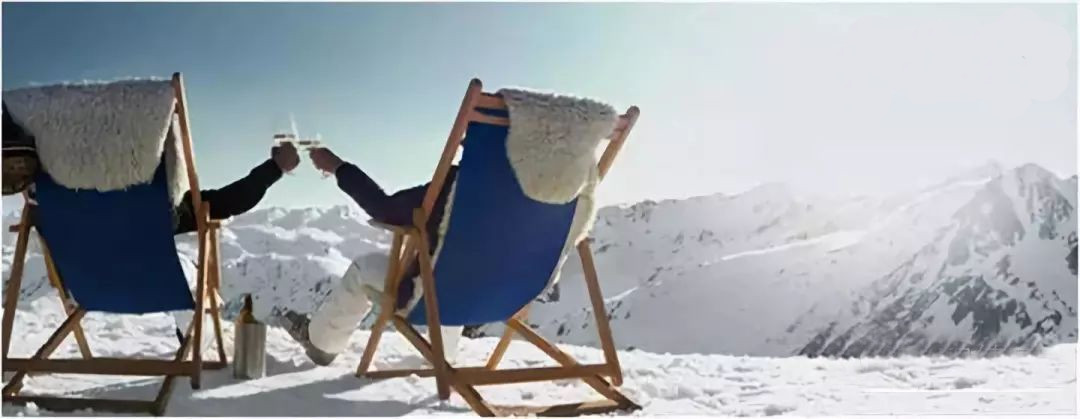
\includegraphics[width=0.6\linewidth]{de_reisen1}
    \caption{德国旅游}
\end{figure}
\paragraph{假日来历:}

“旅游”在全欧或全球范围内都意义重大。对德国人来说,度假可以算最重要的事情之一。人们可以通过度假忘记工作日的疲惫,重新充满能量。“Urlaub(假日)”一词源于中古高地德语“Urloup”。这个词在当时表示上级对某人离开工作岗位的许可。

自1903年起,德国通过带薪休假规定确定了休假天数。那时所有员工都享有三日带薪年休假的权利。早在1841年,德国就出现了由旅游公司Thomas Cook提供的第一个全包旅行。旅客们乘坐火车,从莱斯特到拉夫堡,享受着价格内包含的餐食和乐队演奏等服务。

现在,度假对德国人来说变得更重要了。2013年,全球旅客数量达10.9亿,较2012年增长5\%。旅游行业也得到极大地发展,仅在德国就有300万人从事该行业。



\paragraph{德国假日天数、游客特征:}

现在,德国以年均41天假日和法国在欧洲范围内并列第一,因此德国人和法国人可谓是欧洲的“度假冠军”。就德国而言,除了由雇主保障的30天假日外,在许多联邦州还有额外11天的法定节假日,所以每年德国人常有41天时间供自己随意使用。与之相反,比利时人以年均仅20天带薪假日以及9天法定假日排名垫底。

当德国人出发去度假时,他们当然会做好万全准备。通常来说他们都会带些什么呢?通过什么人们可以一眼就认出德国游客呢?如果德国人准备享受一次火热的夏日风情度假,那么他们首先必备的就是 --- 一顶帽子,帽子可以保护脸部不受阳光暴晒。另外,一个典型德国人在度假时会在脖子上挂一个相机,以便记录下重要的景点风光。穿着方面,他们通常会穿一件衬衫和一条七分裤,必不可少的当然还有一双凉鞋搭配白色袜子。

\paragraph{最受欢迎目的地、住宿方式:}

虽然这有些不可思议,但相比于去别的国家旅游,德国人确实更喜欢留在德国。2015年,像以前一样,德国以29\%这一相当高的比例荣登最受国人喜爱的旅行目的地榜首。2014年,这一比例甚至达到31\%。除此之外德国人也喜欢在欧洲范围内旅行。比如:西班牙以13\%的比例成为最受德国人青睐的国外游目的地,意大利以8.2\%的比例紧随其后。其余较受欢迎的还有奥地利、克罗地亚、希腊和法国等地。

在人们享受应得的假期前,当然得提前订好住宿。那么德国人最喜欢哪种住宿方式呢?对大多数德国人来说,舒服是住宿的第一要义,只有这样他们才能尽可能好地放松,忘记工作日的紧张和压力。另外人们也希望在度假过程中享受到无微不至的服务。所以48\%的德国人选择酒店或舒适的旅馆作为旅行中的过夜地。度假屋以23\%的比例屈居第二。相较起来,帐篷倍受冷落,2015年,只有6\%的德国人选择了此种过夜方式。



\paragraph{度假出行方式:}

在多种不同的出行方式中,开车出行最受德国人青睐,首要原因还在于他们最爱在本国内旅行。因此约有45\%的德国人都喜欢将汽车作为旅行的交通工具。但飞行正行驶在“超车道”上。2015年,约有40\%的德国人乘坐飞机出游。对于前往国外旅游的人,这一比例甚至更高,达到56\%。德国人也会使用公车和铁路交通,不过其占比仅有7\%和5\%。但是现在也有稍稍上升的趋势。相较于国外游,德国人在国内旅游时明显更常使用公车和铁路。



\paragraph{最受喜爱的度假形式\%旅行开销:}

为了能得到尽可能好的休息,德国人特别喜欢在沙滩度假,沙滩之旅以46\%的比例毫无争议拔得头筹。休闲之旅和自然之旅同样也受到他们青睐,分别占比37\%和28\%,差距不大。原则上来说,德国人最爱家庭出游,约有1/4的德国人喜欢和家人一块享受假日。同时探险之旅也很受欢迎,占比24\%,紧随沙滩之旅其后。相反,观光旅行不太受德国人喜爱,仅占比18\%。同样情况的还有徒步旅行,占比17\%。

休假是让人放松的一次奢侈享受,所以德国人用于度假的花费较高。2015年的调查数据显示,如果德国人计划一个5天或更长时间的旅行,平均每人每次旅行的开销为954欧。这一数据较2014年的906欧而言有所升高。平均来看,德国人一次旅行的时间约为12.6天,和2000年相比少了一天。就短期度假旅行而言,德国人一般计划为2到4天,平均每人花销247欧。

\subsubsection{总而言之}

相比于中国人,德国人在旅游有方面更多的追求自由、灵活和探险精神。不同于中国的旅行团的概念,德国人更多的时候以家庭或个人为单位出游。
\subsection{中国的集体主义精神——舍小家,为大家}
\par
新中国成立以来,中国人民为国家建设都有一种舍小家为大家顽强战斗奋力拼搏的精神,留下了许多先进的事迹。最为大家知道的是铁人王进喜,人民公仆焦裕禄等。

\paragraph{铁人王进喜:}
是新中国第一批石油钻探工人,全国著名的劳动模范。他率领钻井队艰苦创业,发扬舍小家顾大家精神,打出来大庆第一块油井,并创造了年进尺10万米的世界钻井记录,为我国石油事业立下汗马功劳。
\paragraph{人民公仆焦裕禄:}
他坚持实事求是、群众路线的领导工作方法,同兰考县全县干部和群众一起,与深重的自然灾害进行顽强斗争,努力改变兰考面貌。他身患肝癌,依旧忍着剧痛,坚持工作,被誉为“党的好干部”、“人民的好公仆”。1964年5月14日,焦裕禄被肝癌夺去了生命,年仅42岁。焦裕禄用自己的实际行动,铸就了亲民爱民、艰苦奋斗、迎难而上、科学求实、无私奉献的焦裕禄精神。
\vspace{1em}
\par
在中国官方的宣传中,上述的这些人物往往作为道德楷模,成为大家学习的榜样。在中国,这样的事迹被认为使人有了一种更高的人生境界,即放弃个人利益,为集体或是全人类的目标而奋斗。因此,集体主义也成为了中国过去几十年激进的社会运动的口号。
%在日常生活中,我们经常可以看见这些宣传标语。这作为一种鼓励我们奋发图强的精神激励着我们努力工作。
\subsection{广场舞}

中国的广场舞起源于中国群众的生活,是一种由人民集体创造的舞蹈形式。它从中国人民群众中来,又到人民群众中去,是一种即具有娱乐意义,同时又兼顾健身锻炼功能的群众自发创造的艺术文化形式。中国广场舞的主要受众是30到50岁之间的中国妇女群众。这些妇女群众就是大家口中著名的中国大妈。中国大妈们十分热爱这项集体运动。她们十数人,或者数十人乃至上百人,集中在空旷的广场上,伴随着具有摇滚和中国特色的流行音乐,跳着步调和节拍一致的舞蹈。而舞蹈的步调与节拍是由大妈们集体商议而来。而种舞蹈的步调与节拍的灵感有的是来自于专业人士的提议,有的则是由大妈们随心随意而作。大家聚集在广场上跳着广场舞,即不需要表现的有多专业,也没有太多规则的束缚。大妈们想来就来,想走就走,想跳就跳。就算大妈们跳错了也不打紧,跳的不好也没人指责。广场舞突出的就是一个集体娱乐性,集体创造性。这种中国式广场舞的文化起点,就是中国集体的农耕文化。中国人习惯了集体活动,在集体中互相帮助,互相学习,共同创造。农耕文化的记忆深深扎根于广大群众的社会生活之中,使得广场舞成为中国人民喜爱的用以宣泄自身情感,展现民族自信,表达民族文化的一种艺术。
\begin{figure}[htb]
    \centering
  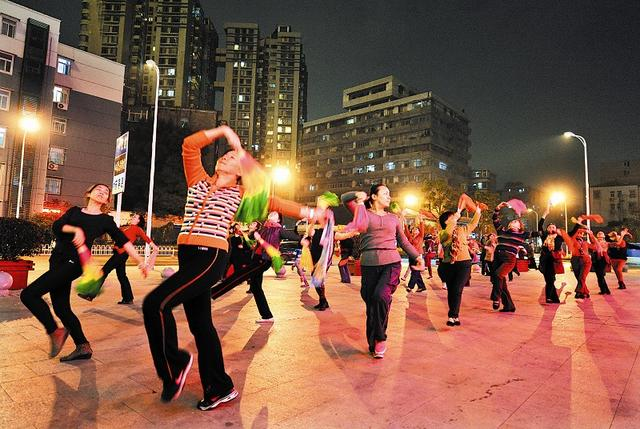
\includegraphics[width=0.6\linewidth]{gcwdm}    
\caption{广场舞大妈}
\end{figure}
\section{中国的传统经济背景}

\subsection{地理环境}

常言道:“知者乐水,仁者乐山。知者动,仁者静。知者乐,仁者寿。” 在中国古代认知中世界就是天圆地方。因为他们认识的只是他们生活的这片土地。虽然中国有着漫长的海岸线,但是很少有人会乘船在海上冒险。在中国古代的各种著作中,谈及海洋时,作者只是赞叹海洋的浩瀚广阔。

相比之下德国的情况就稍有不同了。虽然德国仍有许多地方远离海洋,但就距离而言,和中国的许多地方相比还是比较近的。因此,在比重上德国靠海为生的人更多一些。更关键的是德国在文化上也受到了其它海洋国家的影响,相对而言海洋的味道更浓厚一些。

在德国以及欧洲海岸线犬牙交错,大量的海岛渐渐形成了独立的文化。中国在青藏高原以东的地区的山脉则不是那样难以逾越。中国的中心地带从东到西都有可通航的水系连接起来,而东西则有京杭大运河连接。因此,中国于公元前221年完成统一,就再没有长期分裂过。但欧洲的统一都使欧洲的许多伟人折戟沉沙。

\subsection{中国农业为主的经济环境}

中国历来依靠农业生产来维持生存。在中国历史上,战国时期是中国完成统一的前夕。从那个时期开始每一个封建的小国都把“耕战之术”列为国家要务。直到今日,中国也有近一半的人从事农业生产。在一个以农业为主的国家,最重要的就是土地。对于一个中国人甚至是商人,都是用土地的多寡来体现个人以及家族的财富。因此,在中国历史上,一切社会、经济思想以致政策法律都以土地的分配和利用为核心。


在中国的传统思想中一直有本末之分。对于国家来说,农业生产被认为是立国之本,而商业则是一国之末。因为农业有丰富的产出,而商业只是涉及商品交换,对一个国家物产增加关联较少。
而对于个人来说,读书做官,辅佐君王为本,从事商业活动为末。并且中国人一直推崇“耕读传家”。一般人出身在这样的家庭都会引以为傲。

因此,整个社会中的知识阶层,思想意识上都偏向于农业。对于许多中国古代的官员而言,农业生产也和自己家庭的经济状况相关。这导致中国历史上,各种社会、经济理论以及政策多偏向农业。

\subsection{重农主义的形成}

前面讲到中国农业对于国家的重要性。重农主义也就是我们常说的重农抑商的思想。在中国这一思想在春秋战国时期就已经开始形成了。

\subsubsection{上农}

在中国的吕氏春秋中有一篇叫《上农》的文章,其中比较农民和商人的生活方式。其中认为农民像单纯朴实,惯于顺服,他们的财产以土地为主难以移动。因此国家有难时,农民弃置不顾。商人则奸诈自私,计谋多,他们财产简单,易于转移,因此国家有难是,商人往往自己逃跑,不顾国家。在文中,农业不仅相比于商业对国家更重要,农民的生活方式也更为高尚。

吕氏春秋,反映出中国在春秋战国时期诸子百家,虽然各家思想各有不同,但他们都推崇农民、重视农业。

\subsubsection{汉朝商人地位下降}

汉朝作为中国历史上第一个长期统一的朝代,在之前秦朝的基础上确定了许多中国后来两千年来一直沿用的制度政策。重农抑商就是其中之一。

汉朝创立者高帝命令商人“不得衣丝乘车,重租税以困辱之。”,之后因为天下初得安定,重又放宽对商人的法律,然而商人子孙仍不许当官作吏。但渐渐的,富商大贾蓄积财物,奴役贫民;前呼后拥,车乘百余辆;屯积居奇,地方的诸侯对他们也都伏首低眉,仰仗他们供给物资。有的冶铸煮盐,家财积累到万金,而不帮助国家的急难,黎民百姓陷于重困之中。之后有人就说,商人不从事生产,却囤积居奇,财富越来越多,导致越来越多的人从事商业活动,导致粮食产出的减少。粮食价格上涨,政府发行的货币越来越便宜。所以建议打压商业活动,让商人的财富更多的为国所用。

\subsection{海禁}

中国历史上海禁的高峰期是在明清两朝,不仅在政策上有所强化,而且持续时间长达多年。中国的海禁也成为东南亚陶瓷业发展的契机。另一方面,藩属国例如琉球等国家,亦因为海禁的关系,利用独占与中国贸易的契机而获取大量利益。

清朝海禁政策初期主要是防范郑成功反攻。郑成功等政治势力一直长期依靠海上力量与清朝周旋。康熙时,清朝政府虽然开关与外国贸易,但对外国商船的活动极为注意,对逗留外国的中国人也防范极严。康熙下谕地方官要在沿海各地增设炮台,并指出"海外如西洋等国,千百年后,中国必受其累,国家承平日久,务需安不忘危"。
\paragraph{一口通商}
乾隆二十二年(1757年),乾隆帝南巡,在苏州亲眼目睹洋商船只络绎不绝,引起警觉,导致乾隆对西方殖民活动严加警惕,以海防重地规范外商活动为理由,谕令西洋商人只可以在广东通商,亦即。但是实际上,当时在南洋的一些西方殖民者仍被允许到闽、浙、江海关贸易,特别是闽海关。例如,乾隆四十六年(1781年)、四十八年(1783年)、五十一年(1786年),嘉庆十二年(1807年)、十四年(1809年),均有西班牙商人从南洋吕宋到厦门贸易。

乾隆谕令“本年来船虽已照上年则例办理,而明岁赴浙之船,必当严行禁绝。……此地向非洋船聚集之所,将来只许在广东收泊交易,不得再赴宁波。如或再来,必令原船返棹至广,不准入浙江海口。豫令粤关,传谕该商等知悉。……令行文该国番商,遍谕番商。嗣后口岸定于广东,不得再赴浙省”。 [4]  这一上谕只是让“外洋红毛等国番船”、“番商”只在广东通商,不得再赴浙江等地,而不是一些资料中所说的关闭江、浙、闽三海关,更不是“广州一口通商”。

\subsection{总结}

虽然中国历史上有过对商业活动较为宽松的时期,但是更多的时候,会打压商业活动,制定对商人歧视性的政策。这也是中国历史上不同于德国的特点。

\section{大陆国家和海洋国家}
%section 汉萨同盟
\subsection{汉莎同盟}

\subsection{集权与分权——统一与分裂}

德国历史与中国历史一个很大的区别就是德国长期是由许许多多的小王国或是像汉萨同盟这样的城市组成,他们往往具有独立的军队,政府,相互之前没有隶属关系。中国分裂的时期是短暂的,大部分的时间是在一个集权的中央政府的统治之下。
	\cleardoublepage
\backmatter
\chapter{中德文化补充说明}
	\chapter{资料来源}
\setlength\parindent{0em}
\zihao{-5}
\cnprolight
\mypar
每种语言都有谐音和歧义,为什么唯独中文有这么多象征和禁忌 

\url{https://www.sohu.com/a/229139127_563934} 
\mypar
中国有很多忌讳,你们那里都忌讳什么 

\url{http://baijiahao.baidu.com/s?id=1598772693540609620&wfr=spider&for=pc }
\mypar
祖先不仅留下了很多风俗习惯,还有很多节日禁忌 

\url{https://baijiahao.baidu.com/s?id=1623684014950691097&wfr=spider&for=pc} 
\mypar
中国节日的禁忌,中国人该了解 

\url{https://baijiahao.baidu.com/s?id=1607879372765482140&wfr=spider&for=pc}
\mypar
圣诞节

\url{https://baike.baidu.com/item/%E5%9C%A3%E8%AF%9E%E8%8A%82/127881?fr=aladdin}
\mypar
广场舞

\url{https://baike.baidu.com/item/%E5%B9%BF%E5%9C%BA%E8%88%9E/1445106?fr=aladdin}
\mypar
劝酒

\url{https://wenku.baidu.com/search?word=%C8%B0%BE%C6&ie=gbk}
\mypar
汉莎同盟

\url{https://baike.baidu.com/item/%E6%B1%89%E8%8E%8E%E5%90%8C%E7%9B%9F/7606953?fr=aladdin}
\mypar
宗教改革日

\url{https://baike.baidu.com/item/%E5%AE%97%E6%95%99%E6%94%B9%E9%9D%A9%E6%97%A5/1330418?fr=aladdin}
\mypar
集权与分权——统一与分裂

\url{https://baike.baidu.com/item/%E5%88%86%E5%B0%81%E5%88%B6}
\mypar
中国哲学简史,冯友兰,三联书店

\end{document}